\chapter{SAMBA 4}

O Samba 4 vem com a proposta de criar um \textit{Active Directory} livre, combatendo as versões pagas da Microsoft, utilizando o LDAP, Bind e Kerberos.

Por se tratar de um sistema ainda em fase de produção e sem previsão para a conclusão atualmente, alguns erros podem aparecer ou alguns parâmetros deverão ser modificados. A versão utilizada nesse trabalho é a Alpha22.

Outra coisa, você viu que o Samba 4 já está no 4º Release Candidate... Coloque isso em algum lugar no TCC, pois o projeto já passou dos estados alpha e beta, daqui a pouco será lançado oficialmente como estável...

\section{Instalação do SAMBA 4}

Todos os comandos foram testados no Ubuntu 11.04 e Debian 6, por isso algumas adaptações podem ser necessárias em outras distribuições Linux.

A instalação é realizada a partir do terminal, mas antes é necessário a instalação de algumas bibliotecas.

	\# apt-get install build-essential libattr1-dev libblkid-dev libgnutls-dev python-dev git-core autoconf python-dnspython ntpdate acl libacl1-dev

Antes de começar a instalação o relógio do servidor tem que estar atualizado. O comando ntpdate atualiza a hora através do  ntp\footnote[2]{Os servidores NTP permitem aos seus clientes a sincronização dos relógios de seus computadores e outros equipamentos de rede a partir de uma referência padrão de tempo aceita mundialmente, conhecida como UTC (\textit{Universal Time Coordinated}).\cite{RNP}} , onde um dos principais servidores é o pool.ntp.br.

\# ntpdate pool.ntp.br

O código fonte esta hospedado no servidor git dos desenvolvedores do Samba, e o mesmo deve ser clonado para a maquina de destino.

\# git clone git://git.samba.org/samba.git samba-master; cd samba-master

O Samba 4 segue os procedimento padrões de instalação de aplicativos no linux através do terminal, que segundo \cite{INSTALL} se segue com o ./configure, make e o make install. Nesse caso ao invés de se utilizar o ./configure como padrão é utilizado o ./configure.developer, pois o mesmo habilita alguns modos de debug.

\# ./configure.developer

\# make 

\# make install

Para verificar a versão instalada é só executar o seguinte comando:

\# /usr/local/samba/bin/smbclient "--version


\section{Criação de Domínio com o Samba 4}

O Samba 4 trabalha com regras ACL e para que ele possa ser instalado tem que habilitar o modo acl nas unidades de disco.

\# vim /etc/fstab

Localizar a linha da unidade principal e adicionar o parâmetro acl nos options de montagem da unidade \ref{fstab}.

\begin{figure}[ht]
   	\centering
    \scalebox{1}{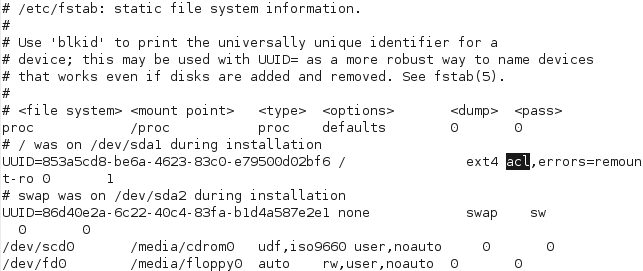
\includegraphics{figuras/fstab}}
   	\caption{Tela do fstab.}
    \label{fstab}
\end{figure}

Por padrão o Samba 4 é instalado no /usr/local/samba.

\# cd /usr/local/samba

A instalação é a partir da execução do comando provision que fica localizado no /sbin do Samba e a inserção de alguns parâmetros.

\noindent \# bin/samba-tool domain provision "--use-ntvfs "--realm=NOME\_SERVIDOR "--domain=NOME DOMINIO  "--adminpass='Senha12' "--server-role=dc

\begin{enumerate}
	\item \textbf{use-ntvfs} - Habilita o NTVFS\footnote[3]{Sistema de arquivos que armazena os atributos do NTFS};
	\item \textbf{realm} - Domínio do servidor Kerberos;
	\item \textbf{domain} - Domínio do Samba;
	\item \textbf{adminpass} - Senha do Administrator, essa senha tem algumas regras de segurança como no mínimo 7 letras uma letra;
	\item \textbf{server-role} - Regra do servidor.
\end{enumerate}

Depois de instalado e configurado o servidor de \textit{Active Directory} pode ser iniciado. Uma das forma é inicia-lo em modo debug para poder acompanhar melhor os processos realizados.

\# /usr/local/samba/sbin/samba -i -M single

Para facilitar a forma de ativar o Samba 4 podem ser feito dois procedimentos.

Criar um link do executável do Samba no /etc/init.d/ .

\# ln /usr/local/samba/sbin/samba /etc/init.d/samba

Mudar o caminho da variável de ambiente PATH para que os comandos possam ser acessados fora da sua pasta de origem.

\# echo ``export PATH=/usr/local/samba/sbin:/usr/local/samba/bin:\$PATH"  $>$$>$ /root/.bashrc

Por padrão o Samba 4 vem com uma servidor interno de DNS, facilitando a criação das zonas e dos mapeamentos. Para a resolução dos nome deve definir o ip da própria maquina como seu dns primário.

\# echo ```domain NOME DOMINIO nameserver IP DO SERVIDOR"  $>$ /etc/resolv.conf

Mesmo contendo um servidor de dns interno o Samba 4 também trabalha com servidores externos, BIND9 versão 9.7 ou mais nova, onde alguns parâmetros de configuração são passados no named.conf.local e named.conf.options para a criação das zonas e atualização automática com o Kerberos.

\# echo 'include ``/usr/local/samba/private/named.conf"' $>$ /etc/bind/named.conf.local

\# vim /etc/bind/named.options

Adicione as seguintes linhas:

\textbf{options}\{ 
	
\textbf{directory ``/usr/local/bind/var/run/named"; }

\textbf{tkey-gssapi-keytab ``/usr/local/samba/private/dns.keytab" ; }

\textbf{tkey-domain ``nome\_do\_realm\_samba"; }
	
\};

As variáveis adicionadas no arquivos são para:

\begin{itemize}
	\item{directory} -  É o caminho absoluto do seu servidor dns;
	\item{tkey-gssapi-keytab} - Local da chave do dns para conexão com o kerberos;
	\item{tkey-domain} - Nome do Domínio.
%	\item{auth-nxdomain} - ...
%	\item{listen-on-v6} - ...
\end{itemize}

\section{Instalação do Kerberos}

Segundo \cite{HEIMDAL} a autenticação Kerberos é um protocolo de rede. Foi concebido para fornecer autenticação forte para o cliente/servidores de aplicativos usando criptografia de chaves secretas, então um cliente pode provar a sua identidade para um servidor (e vice-versa) em uma conexão de rede insegura.
Em nosso caso utilizaremos BIND com suporte ao Heimdal Kerberos por causa do GSS-TSIG algoritmo de serviço de segurança genérico para autenticação de transação com chave secreta de DNS (GSS-TSIG) este mecanismo é utilizado para estabelecer relações TSIG para autenticação do tipo Kerberos, necessário para interagir BIND com Samba 4, com essas credenciais o DNS aceita atualizações GSS-TSIG assinadas e verifica as credenciais de correspondentes com as credencias cadastradas no Samba 4, isso permite aos usuários descarregar o DNS dos usuários do Microsoft Windows sem ter a segurança comprometida.

\begin{itemize}
	\item \textbf{\# apt-get install krb5-user krb5-kdc krb5-config kstart} - Instala todos os pacotes necessários e faz as referências necessárias.
\end{itemize}

Após instalar os pacotes, substitua o /etc/krb5.conf pelo arquivo criado e pré-configurado pelo Samba que esta localizado em /usr/local/samba/private/krb5.conf .

\begin{itemize}
	\item \textbf{\# cp /usr/local/samba/private/krb5.conf  /etc/}
\end{itemize}

Teste para verificar se todos as configurações foram realizadas corretamente.

\begin{itemize}
	\item \textbf{\# host -t SRV \_ldap.\_tcp.``nome do realm sem aspas".} - O resultado deve ser parecido : \textbf{\_ldap.\_tcp.``nome do realm sem aspas" has SRV record 0 100 389 server.``nome do realm sem aspas".}
	\item \textbf{\# host -t SRV \_kerberos.\_udp.``nome do realm sem aspas".} - O resultado deve ser parecido : \textbf{\_kerberos. \_udp.``nome do realm sem aspas" has SRV record 0 100 88 server.``nome do realm sem aspas".}
	\item \textbf{\# host -t A ``nome do realm sem aspas"} - O resultado deve ser parecido : \textbf{``nome do realm sem aspas" has address ``ip do servidor".} 
%	\item \textbf{\# /usr/local/samba/sbin/samba\_dnsupdate "--verbose} - Atualização automática do DNS do Samba.
\end{itemize}

\section{Gerenciando o Samba4 através do Windows e do Linux}

É possível gerenciar o servidor Samba 4 através de um Windows XP mas para a realização do mesmo é necessário a instalação do AdminPack\footnote[4]{O AdminPack está disponível no site da Microsoft:

http://www.microsoft.com/downloads/details.aspx?FamilyID=c16ae515-c8f4-47ef-a1e4-a8dcbacff8e3\&displaylang=en} presente no Windows Server. Essa ferramenta permite gerenciar todos os usuários, grupos e maquinas presentes no \textit{Active Directory}

Inicie a ferramenta pelo \textbf{Executar -$>$ dsa.msc} \ref{tela_dsa}.

\begin{figure}[ht]
   	\centering
    \scalebox{1}{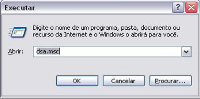
\includegraphics{figuras/dsamsc}}
   	\caption{Tela para executar o DSA.}
    \label{dsa}
\end{figure}
 
%\pagebreak

\begin{figure}[h!]
   	\centering
    \scalebox{1}{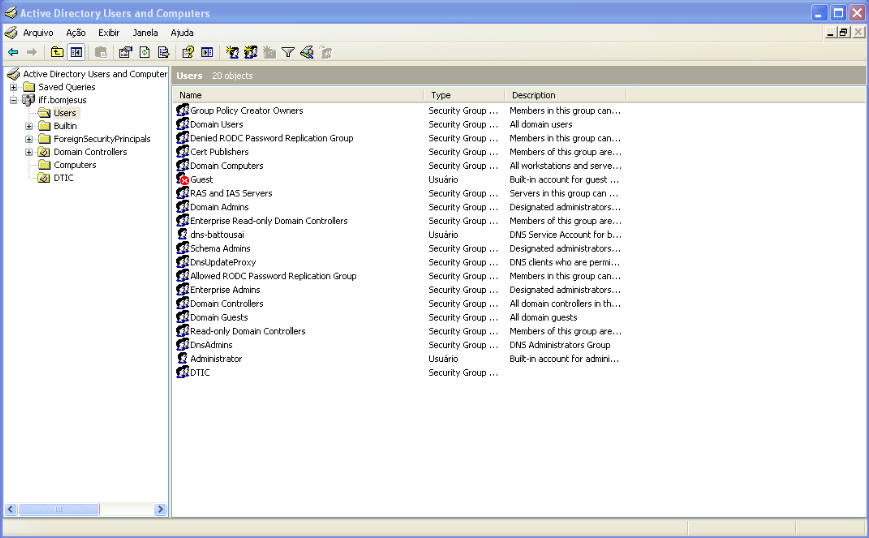
\includegraphics{figuras/addsa}}
   	\caption{Tela do DSA.}
    \label{tela_dsa}
\end{figure}

\pagebreak

O samba-tools é uma ferramenta que acompanha o Samba 4 no linux e tem a finalidade de gerenciar as ações que podem ser feitas no no \textit{Active Directory}. Com ele se poder criar usuários, grupos, gpo's, entre outras funções, porém um forma de texto \ref{samba-tool}.

\begin{figure}[h!]
   	\centering
    \scalebox{1}{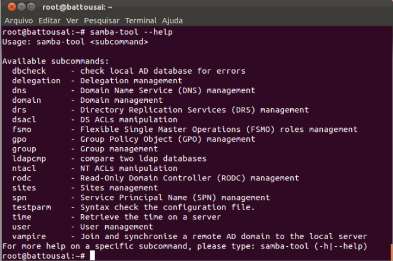
\includegraphics{figuras/samba-tool}}
   	\caption{samba-tool no terminal.}
    \label{samba-tool}
\end{figure}

%\pagebreak

%\section{Compartilhamento de arquivos e impressoras}

%SAMBA4 ainda não consegue compartilhar arquivos e impressoras de forma fácil e simplificada como o Samba 3, e tem problemas com a integração dos usuários e grupos do \textit{Active Directory} com os locais, dificultando a definição das permissões a arquivos e diretórios.

%Uma solução para tal problema é identificar o código do usuário no \textit{Active Directory} e dar as devidas permissões a pasta desejada.

%\begin{itemize}
%	\item \textbf{\# /usr/local/samba/bin/wbinfo "--name-to-sid USERNAME} - O resultado deve ser o sid do usuário no Samba. Exemplo : S-1-5-21-4036476082-4153129556-3089177936-1005 SID\_USER(1).
%	\item \textbf{\# /usr/local/samba/bin/wbinfo "--sid-to-uid S-1-5-21-4036476082-4153129556-3089177936-1005} - Mostra o id do usuário e é a referência do usuário local com o do Samba 4.
%	\item \textbf{\# chown 3000011 /pasta\_que\_será\_compartilhada} - Mudando o usuário do diretório e as suas permissões, o usuário do AD irá ter o acesso aos arquivos.
%\end{itemize} 

\section{Maquinas linux interagindo com o \textit{Active Directory} do  Samba4}

Segundo \cite{UBUNTU-WIKI} a forma de incluir uma maquina Ubuntu no \textit{Active Directory} é modificar alguns arquivos de configuração.Segue abaixo os arquivos e os procedimentos.

\textbf{Informações}

\begin{itemize}
	\item \textbf{fja.br} -  Domínio do \textit{Active Directory}.
	\item \textbf{fjadc01.fja.br} - Controlador de domínio.
	\item \textbf{10.1.0.1} - IP do controlador de domínio.
	\item \textbf{FJA.BR} - Kerberos Realm.
	\item \textbf{gert} - Estação de Trabalho Ubuntu.
	\item \textbf{gert.fja.br} - FQDN da estação de trabalho.
	\item \textbf{fjadc01} - Servidor NTP.
\end{itemize}

\textbf{Instalando os pacotes necessários}

\begin{itemize}
	\item {\# aptitude install krb5-user libpam-krb5 winbind samba smbfs smbclient krb5-config libkrb53 libkadm55 vim}
\end{itemize}

\textbf{Sincronizando a hora}

\begin{itemize}
	\item {\# ntpdate 10.2.0.1}
\end{itemize}

\textbf{Edite o arquivo /etc/hosts adicionando o ip e o nome do DC de sua rede.}

\begin{itemize}
	\item {\# vim /etc/hosts}
\end{itemize}

127.0.0.1       gert.fja.br localhost gert

127.0.1.1       gert

\# The following lines are desirable for IPv6 capable hosts

::1     ip6-localhost ip6-loopback

fe00::0 ip6-localnet

ff00::0 ip6-mcastprefix

ff02::1 ip6-allnodes

ff02::2 ip6-allrouters

ff02::3 ip6-allhosts

10.2.0.1   fjadc01

10.2.0.2   fjadc02

\textbf{Configurando o Kerberos}

\begin{itemize}
	\item {\# vim /etc/krb5.conf}
\end{itemize}

[libdefaults]

	default\_realm = FJA.BR

[realms]

    FJA.BR = \{

      kdc = fjadc01.fja.br

      default\_domain = FJA.BR

      kpasswd\_server = fjadc01.fja.br

      admin\_server = fjadc01.fja.br

     \}

[domain\_realm]

.fja.br = FJA.BR

\textbf {Testando a conexão com o \textit{Active Directory}.}

\begin{itemize}
	\item {kinit $<$ENTER$>$}
	\item {Password for alex$@$FJA.BR: ****}
	\item {klist $<$ENTER$>$}
	\item {Ticket cache: FILE:/tmp/krb5cc\_1000}
	\item {Default principal: alex$@$FJA.BR}
\end{itemize}

\textbf {Se o resultado for este o Kerberos está funcionando corretamente.}

	Valid starting Expires Service principal 07/16/07 15:48:35  07/17/07 01:49:08  

	krbtgt/FJA.BR@FJA.BR renew until 07/17/07 15:48:35
	
	Kerberos 4 ticket cache: /tmp/tkt1000
	
	klist: You have no tickets cached

\textbf{Acessando o Domínio.}

\begin{itemize}
	\item {\# vim /etc/samba/smb.conf} -  Adicione as seguintes linhas.
\end{itemize}

[global]

        security = ads

        realm = FJA.BR

        password server = 10.2.0.1

        workgroup = ADMINISTRATIVO

\#       winbind separator = +

        idmap uid = 10000-20000

        idmap gid = 10000-20000

        winbind enum users = yes

        winbind enum groups = yes

        template homedir = /home/\%D/\%U

        template shell = /bin/bash

        client use spnego = yes

        client ntlmv2 auth = yes

        encrypt passwords = yes

        winbind use default domain = yes

        restrict anonymous = 2

\# to avoid the workstation from

\# trying to become a master browser

\# on your windows network add the

\# following lines

        domain master = no

        local master = no

        preferred master = no

        os level = 0

\textbf{Reinicie os serviços.}

\begin{itemize}
	\item \textbf{\# /etc/init.d/winbind stop}
	\item \textbf{\# /etc/init.d/samba restart}
	\item \textbf{\# /etc/init.d/winbind start}
\end{itemize}

\textbf{Adicione a conta ao domínio.}

\begin{itemize}
	\item \textbf{\# net ads join}
	\item \textbf{Resultado} - Using short domain name – GERT Joined ``GERT" to realm ``FJA.BR"
\end{itemize}

\textbf{Configure a Autenticação.}

\begin{itemize}
	\item \textbf{\# vim /etc/nsswitch.conf}
\end{itemize}

	passwd:         compat winbind

	group:          compat winbind

	shadow:         compat

\textbf{Teste o winbind}

\begin{itemize}
	\item {getent passwd}
\end{itemize}

quiosque:*:10018:10000:Quiosque:/home/ADMINISTRATIVO/quiosque:/bin/bash

\begin{itemize}
	\item {getent group}
\end{itemize}

\_\_coordenação de enfermagem:x:10046:coordenf

\_\_coordenação de design:x:10047:smarino,coorddes

\textbf{Configure o PAM.}

\begin{itemize}
	\item {\# vi /etc/pam.d/common-account} - Adicione as seguintes linhas.
\end{itemize}

account sufficient       pam\_winbind.so

account required         pam\_unix.so

\begin{itemize}
	\item {\# vim /etc/pam.d/common-auth} - Adicione as seguintes linhas.
\end{itemize}

auth sufficient pam\_winbind.so

auth sufficient pam\_unix.so nullok\_secure use\_first\_pass

auth required   pam\_deny.so

\begin{itemize}
	\item {\# vim /etc/pam.d/common-session} Adicione as seguintes linhas.
\end{itemize}

session required pam\_unix.so

session required pam\_mkhomedir.so umask=0022 skel=/etc/skel

\begin{itemize}
	\item {/etc/pam.d/sudo} - Adicione as seguintes linhas.
\end{itemize}

auth sufficient pam\_winbind.so

auth sufficient pam\_unix.so use\_first\_pass

auth required   pam\_deny.so

$@$include common-account

\textbf{Reinicie os serviços}

\begin{itemize}
	\item \textbf{\# /etc/init.d/winbind stop}
	\item \textbf{\# /etc/init.d/samba restart}
	\item \textbf{\# /etc/init.d/winbind start}
\end{itemize}

\textbf{Logando no domínio.}

Vá para a console usando o comando CTRL+ALT+F1 e logue no sistema com o login e senha do domínio.

\begin{itemize}
	\item {login: nome\_do\_usuário}
	\item {Password: *****}
	\item {nome\_do\_usuário$@$gert:~\$}
\end{itemize}

\section{Script para adicionar maquina linux no \textit{Active Directory}.}

O cadastro de maquinas no samba 4 se difere do samba 3 por não ser necessário o cadastramento do computador como usuário, com o \$ no final do nome, no servidor e depois cadastra-lo no Samba 4.

Para facilitar a inserção das maquinas linux no \textit{Active Directory} do Samba 4 foi modificado um script e ele foi chamado de smbad.sh\footnote[4]{Pode ser baixado em https://github.com/GabrielRocha/Monografia/blob/master/latex/Scripts/smbad.sh}. 

\begin{figure}[ht]
   	\centering
    \scalebox{1}{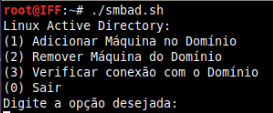
\includegraphics{figuras/smbad}}
   	\caption{Tela do script para inserir maquinas linux no AD.}
    \label{smbad}
\end{figure}

\section{Samba3 e Samba 4}

%O Samba 3 e Samba 4 não podem ser instalados e configurados no mesmo servidor por trabalharem com os mesmos daemons de inicialização, um serviço quando iniciado anula o outro.

%Por ainda terem funções distintas a melhor forma de se trabalhar com os dois na mesma rede é trabalhando em servidores distintos porém interligados. 

%O servidor onde o Samba 3 estiver instalado terá que ser cadastrado no servidor Samba 4 para poder fazer o login a partir dele, assim todas as regras feitas no Samba 3 em relação a permissão de usuário no compartilhamento serão validas para os usuários cadastrados no Samba 4.

\section{Windows no domínio Samba 4}